\begin{frame}{\og{}Rupture\fg{} épistémologique {\small(\hypersetup{citecolor=yellow}\cite{bachelard1993formation})}}
\begin{itemize}
\item \og{}révolution scientifique\fg{} {\small(\cite{koyre1962monde})}
\item \og{}changement de paradigme\fg{} {\small(\cite{kuhn1962structure})} 
\end{itemize} 
\begin{figure}
    \centering
    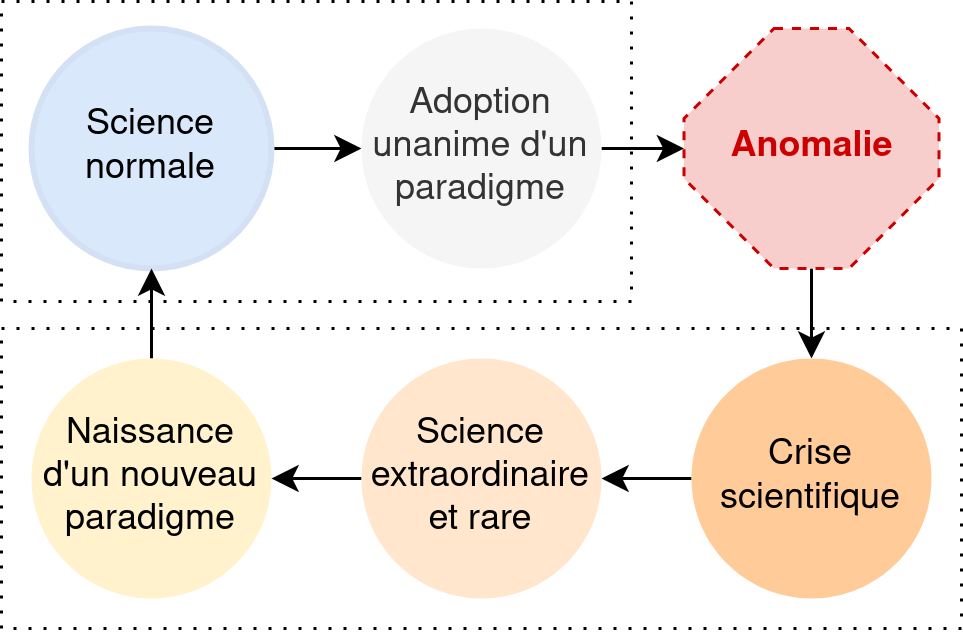
\includegraphics[width=75mm,scale=0.5]{pic/doxa_episteme.png}
    \caption{Conception kuhnienne du progrès scientifique, adaptée de {\small\textcite{amiri}}.}
    \label{fig:enter-label}
\end{figure}
\end{frame}



